\documentclass[11pt,a4paper]{article}
\usepackage[a4paper, total={7in, 10.25in}]{geometry}


\usepackage{color}
\usepackage{graphicx}
\usepackage{wrapfig}
\usepackage{fancyhdr}
\usepackage{tocloft}
\usepackage{multicol}
\usepackage{hyperref}
\usepackage{tabularx}
\usepackage{array}
\usepackage[export]{adjustbox}
\usepackage{listings}
\usepackage{xcolor}
    \definecolor{codegreen}{rgb}{0,0.6,0}
    \definecolor{codegray}{rgb}{0.5,0.5,0.5}
    \definecolor{codepurple}{rgb}{0.58,0,0.82}
    \definecolor{backcolour}{rgb}{1,1,1}

    \lstdefinestyle{mystyle}{
        backgroundcolor=\color{backcolour},   
        commentstyle=\color{codegreen},
        keywordstyle=\color{magenta},
        numberstyle=\tiny\color{codegray},
        stringstyle=\color{codepurple},
        basicstyle=\ttfamily\footnotesize,
        breakatwhitespace=false,         
        breaklines=true,                 
        captionpos=b,                    
        keepspaces=false,                 
        numbers=left,                    
        numbersep=5pt,                  
        showspaces=false,                
        showstringspaces=false,
        showtabs=false,                  
        tabsize=2
    }



\renewcommand{\cftsecleader}{\cftdotfill{\cftdotsep}}
\graphicspath{ {./images/} }
\hypersetup{
    colorlinks=true,
    linkcolor=blue,
    citecolor=black,
    filecolor=magenta,      
    urlcolor=cyan,
    pdftitle={Overleaf Example},
    pdfpagemode=FullScreen,
    }
\pagestyle{fancy}
\setlength{\headheight}{18pt}
\fancyhead[L]{\textit{EN3160 Image Processing and Machine Vision : Assignment 01}}
\fancyfoot[L]{\textit{Department of Electronic and Telecommunication \\University of Moratuwa}}

\title{DEPARTMENT OF ELECTRONIC AND TELECOMMUNICATION
UNIVERSITY OF MORATUWA

\vspace{10pt}

{\large{\textsc{EN 3160: Image Processing and Machine Vision}}}

{\textsf{This is offered as a "EN 3160: Image Processing and Machine Vision" module's partial completion.}}

\vspace{30pt}

\includegraphics[scale=1.20]{images/University_of_Moratuwa_logo.png}

{\textsf{\textbf{Assignment 01}}}}


\author{200686J : Vishagar A.}

\date{$29^{th}$ of august, 2023}

\begin{document}

\maketitle

\newpage

\begin{abstract}

    \textit{This report deals with the procedure of solving each set of problems provided for our assignment. This includes the theoretical approach for each question and implementation of those approaches for real world images. These questions deal with many important basic image processing techniques like intensity transformation, spatial filtering, gamma correction, histogram equalization and much more.}
\end{abstract}    

\vspace{50pt}
\tableofcontents


\newpage

\twocolumn

\section{Question 01}
Question one deals with intensity transformation for a image. Our task is to do a intensity transformation for a given image. The intensity transformation function was also given. An intensity transformation is a technique that maps each intensity value of an input image to a corresponding output intensity value through a mathematical expression.

\lstset{style=mystyle}
\lstinputlisting[language=Octave]{code1.py}

{\begin{figure}[h]
    \centering
    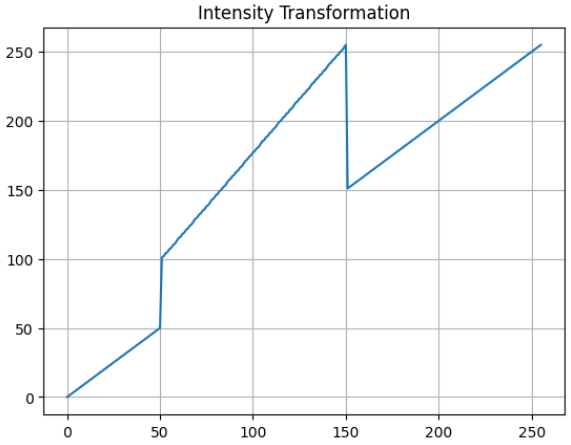
\includegraphics[width=0.7\linewidth]{images/intensity_transformer.png}
    \caption{Intensity Transformer}
\end{figure}}

{\begin{figure}[h]
    \centering
    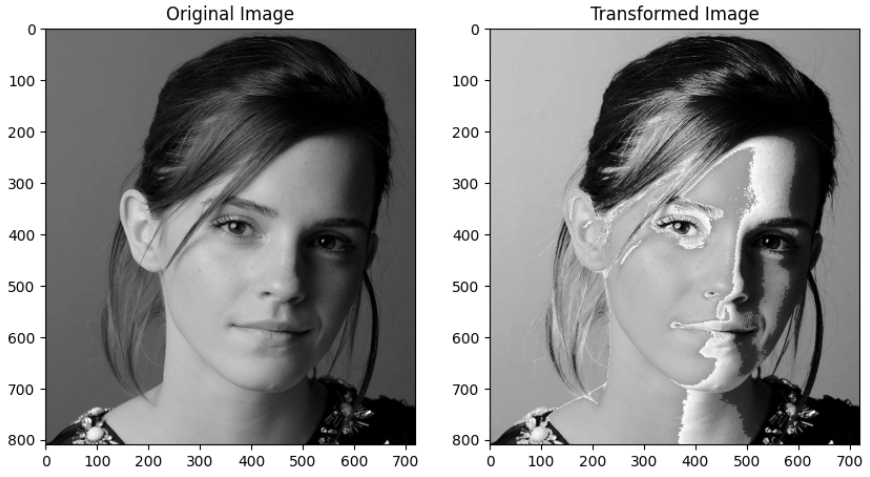
\includegraphics[width=0.9\linewidth]{images/emma.png}
    \caption{Result after Intensity Transformation}
\end{figure}}

\newpage

\section{Question 02}
Question2 deals with intensity transformers as in question one, but here particularly we were asked to accentuate gray and white matters in a brain proton density image. In range of intensities from 50 to 180 gray matter got accentuated and from 180 to 255 white matter got accentuated.

{\begin{figure}[h]
    \centering
    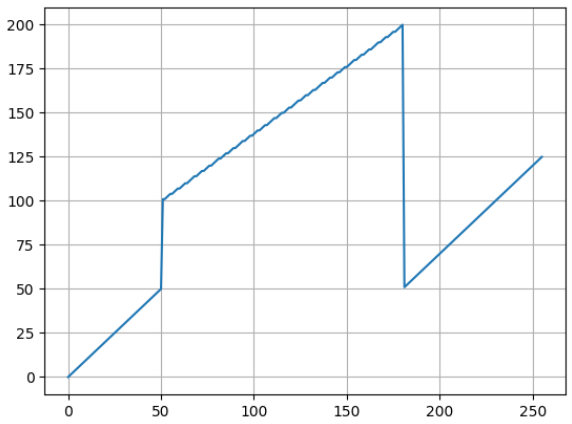
\includegraphics[width=0.8\linewidth]{images/intensity_transformer2.png}
    \caption{Intensity Transformer}
\end{figure}}

{\begin{figure}[h]
    \centering
    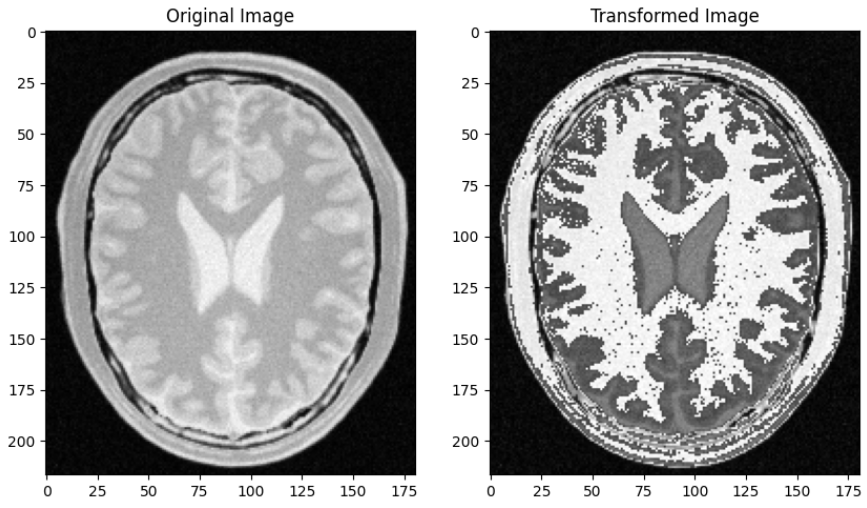
\includegraphics[width=0.9\linewidth]{images/gray_matter.png}
    \caption{Accentuated gray matter}
\end{figure}}

{\begin{figure}[h]
    \centering
    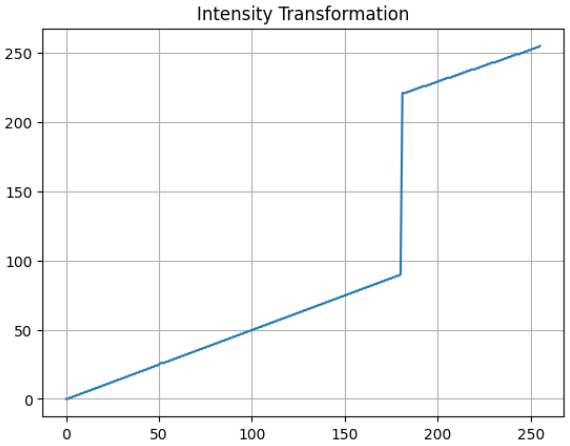
\includegraphics[width=0.8\linewidth]{images/intensity_transformer3.png}
    \caption{Intensity Transformer}
\end{figure}}

\newpage

\begin{figure}[h]
    \centering
    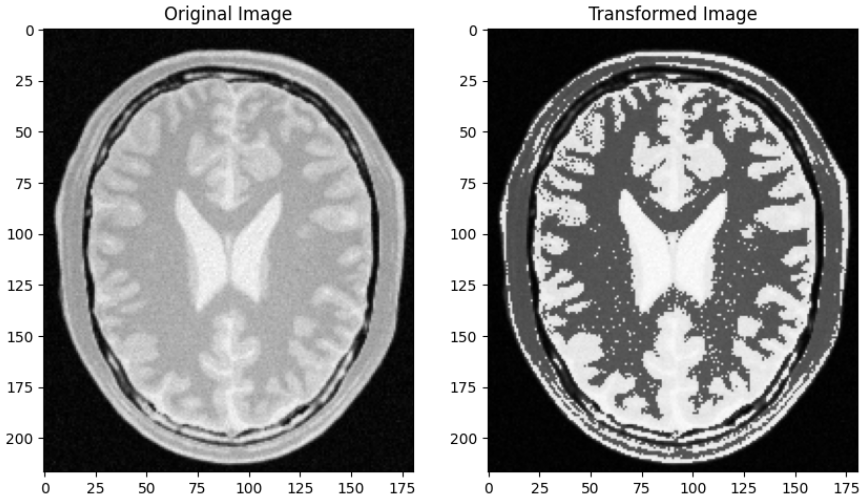
\includegraphics[width=0.9\linewidth]{images/white_matter.png}
    \caption{White Matter}
\end{figure}

\section{Question 03}

In Question 3 we were asked to perform gamma correction particularly for L plan from (L,a,b) categories. Here we are applying a gamma correction for lightness (L) plane to increase and enhance the brightness of the image.
\lstset{style=mystyle}
\lstinputlisting[language=Octave]{code3.py}

\newpage

{\begin{figure}[h]
    \centering
    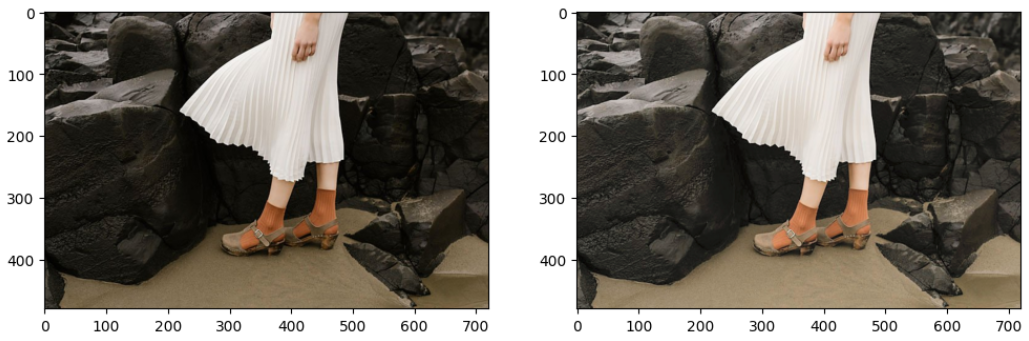
\includegraphics[width=1.0\linewidth]{images/gamma.png}
    \caption{Gamma Corrected Image}
\end{figure}}

\section{Question 04}

In this question we were asked to do a intensity transformation in a particular image plane ( Saturation ) extracted from hue,saturation and value planes to enhance tha vibrancy of the images.

\lstset{style=mystyle}
\lstinputlisting[language=Octave]{code4.py}

{\begin{figure}[h]
    \centering
    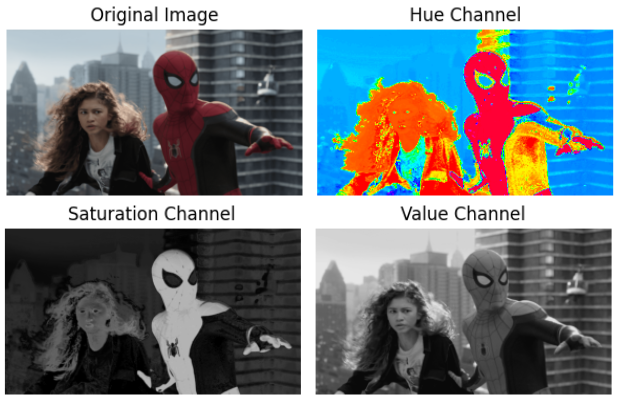
\includegraphics[width=1.0\linewidth]{images/4.png}
    \caption{Hue,Saturation and Value Planes}
\end{figure}}

\newpage

\section{Question 05}

In this question we were asked to carry out histogram equalization but without using \textbf{cv2.equihist()} option. Alternate method in the slides was implemented.

\lstset{style=mystyle}
\lstinputlisting[language=Octave]{code5.py}

{\begin{figure}[h]
    \centering
    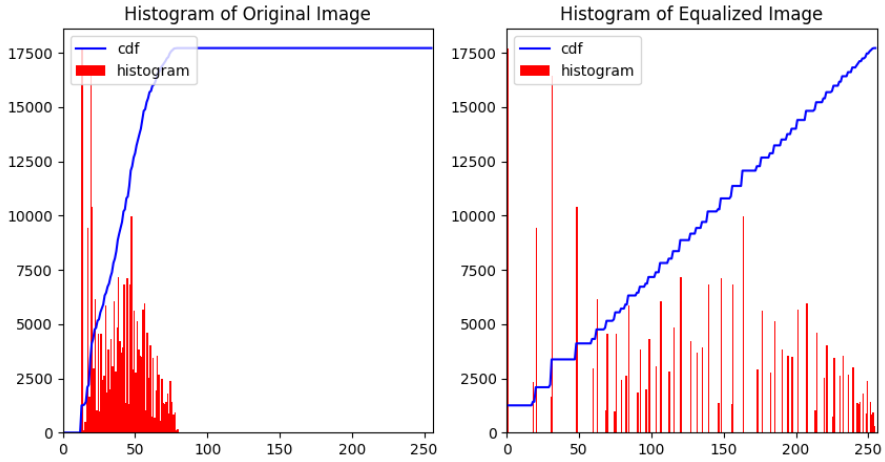
\includegraphics[width=1\linewidth]{images/5-1.png}
    \caption{Equalized Histogram}
\end{figure}}

\newpage

{\begin{figure}[h]
    \centering
    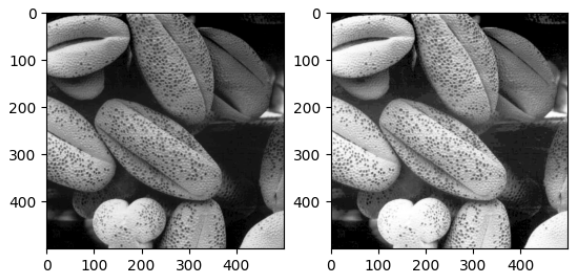
\includegraphics[width=1\linewidth]{images/5-2.png}
    \caption{Histogram Corrected Image}
\end{figure}}

\section{Question 06}

In this question we were asked to split the image in to hue,saturation and value planes , visulaize it and find a mask to extract the foreground and background from the image and do histogram equalization for the foreground and enhance the image.

{\begin{figure}[h]
    \centering
    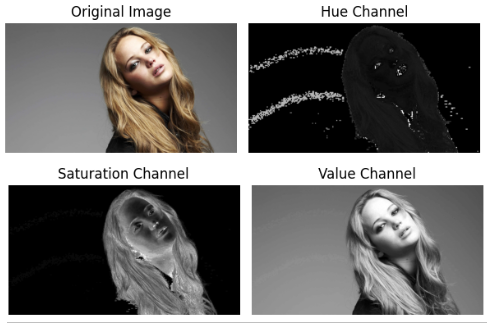
\includegraphics[width=1\linewidth]{images/6-1.png}
    \caption{Hue Saturation and Value Planes}
\end{figure}}

{\begin{figure}[h]
    \centering
    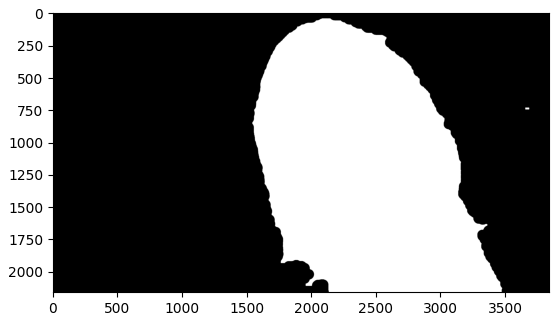
\includegraphics[width=1\linewidth]{images/6-2.png}
    \caption{Mask}
\end{figure}}

\newpage

\lstset{style=mystyle}
\lstinputlisting[language=Octave]{code6.py}

{\begin{figure}[h]
    \centering
    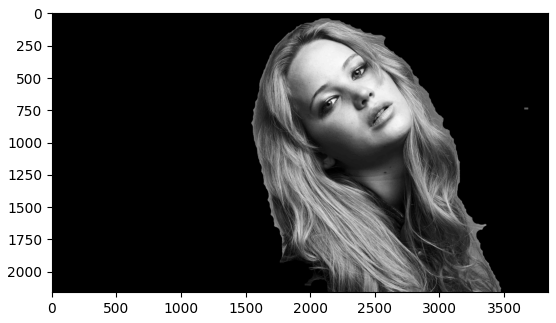
\includegraphics[width=0.9\linewidth]{images/6-3.png}
    \caption{Extracted foreground}
\end{figure}}

{\begin{figure}[h]
    \centering
    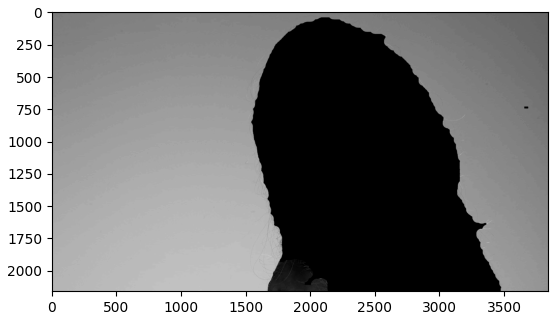
\includegraphics[width=0.9\linewidth]{images/6-5.png}
    \caption{Extracted background}
\end{figure}}

{\begin{figure}[h]
    \centering
    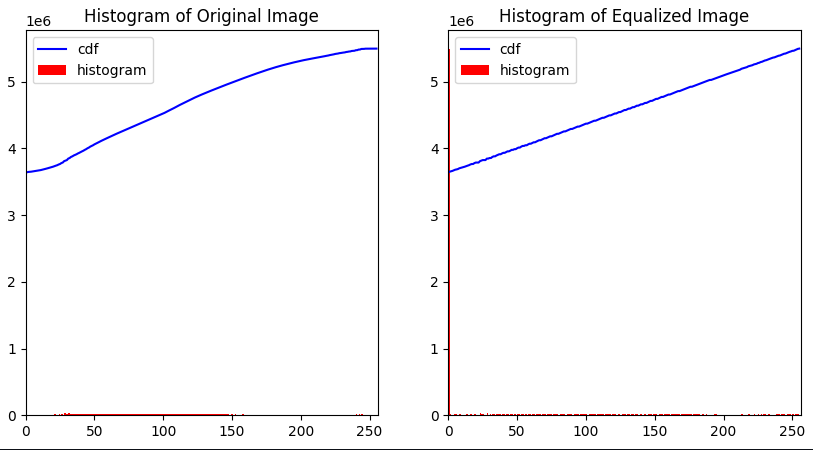
\includegraphics[width=0.9\linewidth]{images/6-4.png}
    \caption{Histogram Correction}
\end{figure}}

\newpage

{\begin{figure}[h]
    \centering
    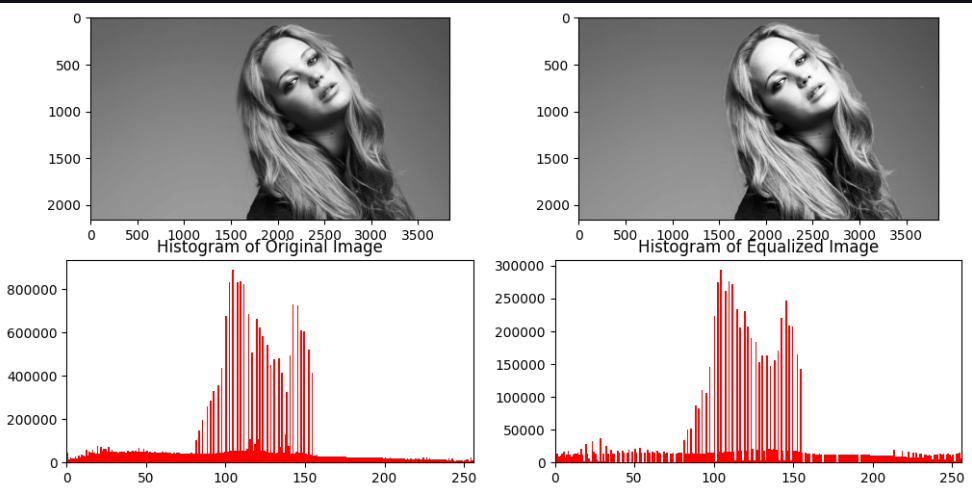
\includegraphics[width=1\linewidth]{images/6-6.png}
    \caption{Histogram Corrected Image}
\end{figure}}



\section{Question 07}

In this section we were asked to perform sobel filtering for a given image and find the gradient magnitude using three different approaches. Normally sobel filter is used to detect the vertical and horizontal edges or gradients of an image. Therefore sobel filters are generally called as ``Sobel Horizontal'' and ``Sobel Vertical''. with their respective kernels.How ever in this question we were asked to use the given kernel therefore I have computed the respective gradient and sobel filtered image for the given kernel.


\subsection{Using Buit-in Filter2D function}
\lstset{style=mystyle}
\lstinputlisting[language=Octave]{code71.py}

{\begin{figure}[h]
    \centering
    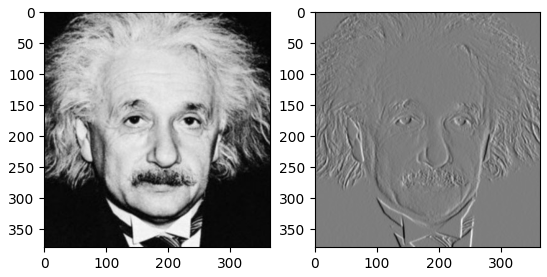
\includegraphics[width=1\linewidth]{images/7-1.png}
    \caption{Gradient Magnitude using Filter2D}
\end{figure}}
\newpage

\subsection{Using Iterations}

\lstset{style=mystyle}
\lstinputlisting[language=Octave]{code72.py}

{\begin{figure}[h]
    \centering
    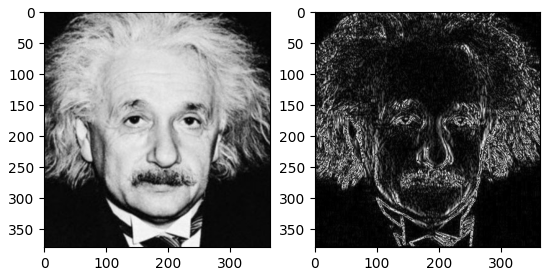
\includegraphics[width=1\linewidth]{images/7-2.png}
    \caption{Gradient Magnitude using Iterations}
\end{figure}}


\subsection{Using multiplication of two kernels}
\lstset{style=mystyle}
\lstinputlisting[language=Octave]{code73.py}

{\begin{figure}[h]
    \centering
    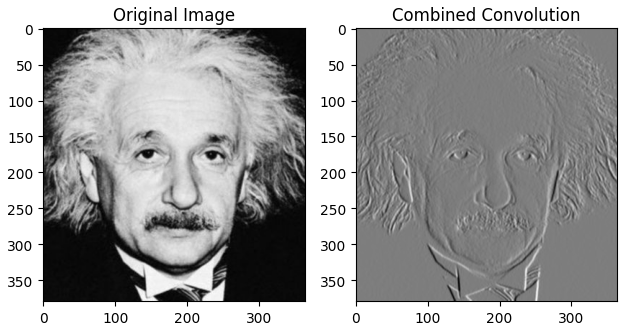
\includegraphics[width=1\linewidth]{images/7-3.png}
    \caption{Gradient Magnitude using Multiplication}
\end{figure}}

\newpage

\section{Question 08}

In this question we were asked to zoom an image using nearest neighbout and bilinear interpolation methods. Nearest neighbour interpolation is a simple method in which the value of the new pixel is determined by the value of the nearest pixel in the original image. Bilinear interpolation is a more complex method in which the value of the new pixel is determined by the weighted average of the 4 nearest pixels in the original image.

\lstset{style=mystyle}
\lstinputlisting[language=Octave]{code8.py}


{\begin{figure}[h]
    \centering
    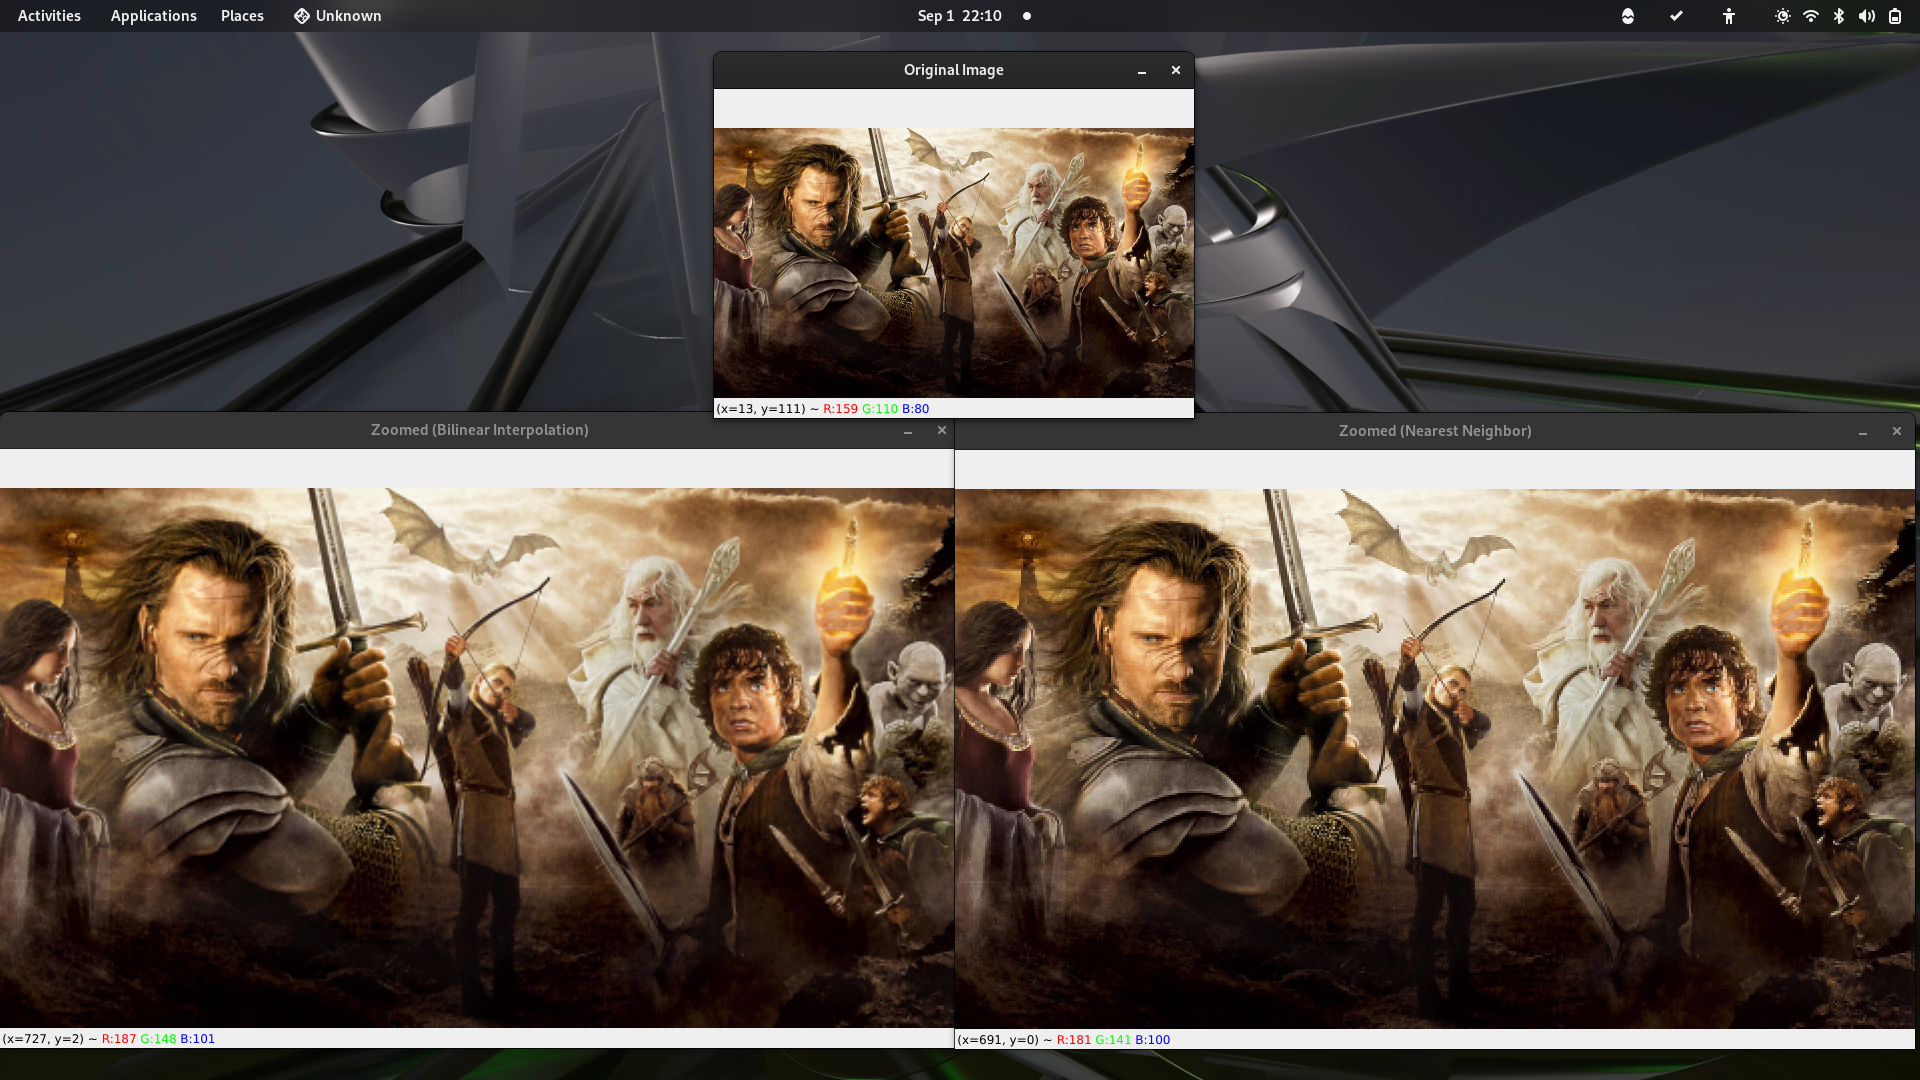
\includegraphics[width=1\linewidth]{images/7-4.png}
    \caption{Zooming of an image}
\end{figure}}

\section{Question 09}

In this question we were asked to come over a mask to extract the foreground from a given image and apply a gaussian filter to the extracted background to make it blur. 

\lstset{style=mystyle}
\lstinputlisting[language=Octave]{code9.py}

\newpage

{\begin{figure}[h]
    \centering
    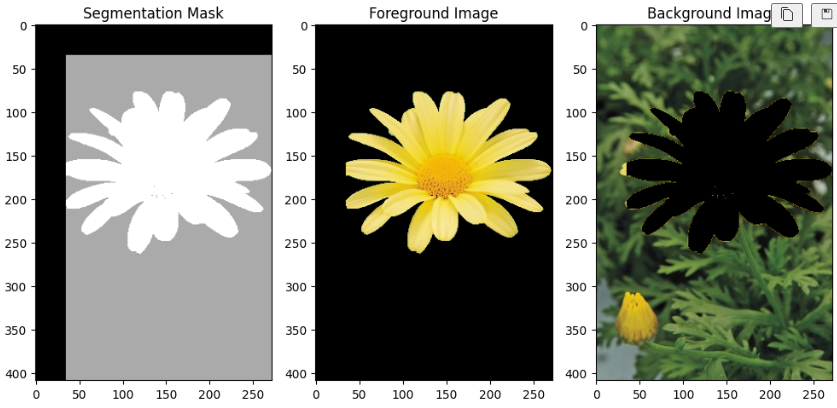
\includegraphics[width=1\linewidth]{images/9-1.png}
    \caption{Mask and extraction of foreground and background}
\end{figure}}

{\begin{figure}[h]
    \centering
    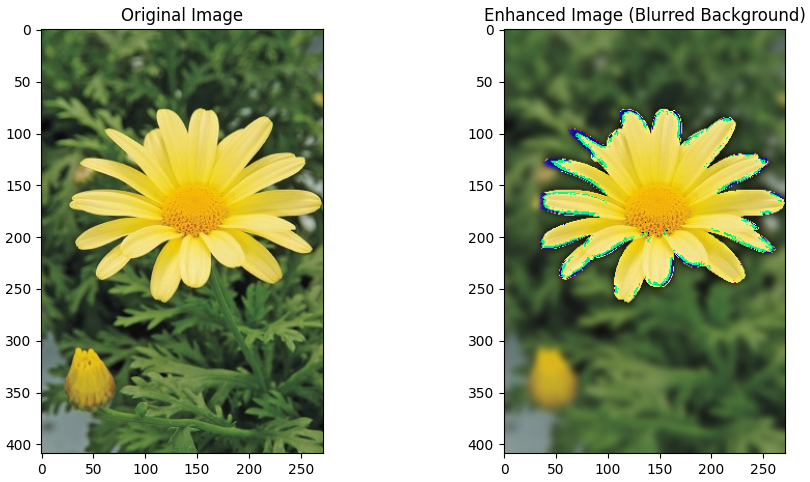
\includegraphics[width=1\linewidth]{images/9-2.png}
    \caption{Blurred background and result}
\end{figure}}


\section{References}

\begin{itemize}
    \item \href{https://opencv.org/}{OpenCV Documentation}
    \item \href{https://www.youtube.com/@RangaRodrigo}{Youtube Resources}
    % \item \href{ }{Github/EN3160_Assignment_01}
   
\end{itemize}

\section{Github Repository}

Following is the link to my Github repository for this assignment.\\

\href{https://github.com/Vgr20/EN3160Assignment01.git }{Github/EN3160\_Assignment\_01}




\end{document}




%%%%%%%%%%%%%%%%%%%%%%%%%%%%%%%%%%%%%%%%%%%%%%%%%%%%%%%%%%%%%%%%%%%%%%%%%%%%%%%%%%%%%%%%%%%%%%%%%%%%%%%%%%%%%%%%%%%%%%%%%%%%%%%%%%%%%%%%%%%%%%%%%%%%%%%%%%%%%%%%%%%%%%%%%%

% {\begin{center}
% \begin{tabular}{ | m{1.85cm} | m{0.85cm}| m{0.85cm} | m{0.85cm} | m{0.85cm} | m{0.85cm} | } 
%  \hline
%  Objectives& Weight & Design 01 & Design 02 & Design 03 & Design 04 \\  
%  \hline\hline
%  Efficiency & 10 & 7 & 8 & 8 & 9 \\
%  \hline
%  Mobility & 10 & 7 & 9 & 8 & 8 \\
%  \hline
%  Easy Maintenance & 10 & 7 & 6 & 5 & 8 \\
%  \hline
%  Refilling accessibility & 5 & 3 & 3 & 2 & 4 \\
%  \hline
%  Durability & 5 & 2 & 3 & 3 & 2 \\
%  \hline
%  Manufacture cost & 5 & 3 & 3 & 2 & 3 \\
%  \hline
%  Overall Look & 5 & 2 & 3 & 5 & 2 \\
%  \hline
%  \hline
%  Total & 50 & 31 & 35 & 33 & 36 \\
%  \hline
 
% \end{tabular}
% \end{center}}

%%%%%%%%%%%%%%%%%%%%%%%%%%%%%%%%%%%%%%%%%%%%%%%%%%%%%%%%%%%%%%%%%%%%%%%%%%%%%%%%%%%%%%%%%%%%%%%%%%%%%%%%%%%%%%%%%%%%%%%%%%%%%%%%%%%%%%%%%%%%%%%%%%%%%%%%%%%%%%%%%%%%%%%%%%


% \begin{center}
% \begin{tabular}{ | m{2cm} | m{5cm}| m{2cm} | m{6cm} | } 

%  \hline
%  Part Name & Description & Supplier & Part Link\\  
%  \hline\hline
%  NE555P & 8-pin Precise timer & Texas Instruments & \href{https://www.lcsc.com/product-detail/Timers-Clock-Oscillators_Texas-Instruments-NE555P_C46749.html}{NE555p data sheet}\\
%  \hline
%  2N2222A & Generic npn transistor & Slkor & \href{https://www.lcsc.com/product-detail/Bipolar-Transistors-BJT_Slkor-SLKORMICRO-Elec-2N2222A_C5330385.html}{2N2222A data sheet}\\
%  \hline
%   LM7805 & Linear voltage Regulators & LRC & \href{https://www.lcsc.com/product-detail/Linear-Voltage-Regulators-LDO_LRC-LR7805_C2846986.html}{Lm7805 Data sheet}\\
%  \hline
%   HC sr501 & Passive IR sensor & HC & \href{https://www.lcsc.com/product-detail/Timers-Clock-Oscillators_Texas-Instruments-NE555P_C46749.html}{HC sr501 data sheet}\\
%  \hline
%   KNSCHA ZE11000UF & 1000uF Capacitor & KNSCHA & \href{https://www.lcsc.com/product-detail/Solid-Capacitors_KNSCHA-ZE11000UF35V119EC0014_C2992586.html}{Capacitor data sheet}\\
%  \hline
%   Resistors & Resistors with different values & Texas Instruments & \href{https://www.lcsc.com/search?q=resistors%20through%20hole}{Through hole resistors}\\
%  \hline
 
% \end{tabular}  
% \end{center}
%%%%%%%%%%%%%%%%%%%%%%%%%%%%%%%%%%%%%%%%%%%%%%%%%%%%%%%%%%%%%%%%%%%%%%%%%%%%%%%%%%%%%%%%%%%%%%%%%%%%%%%%%%%%%%%%%%%%%%%%%%%%%%%%%%%%%%%%%%%%%%%%%%%%%%%%%%%%%%%%%%%%%%%%%%
